% Every table below is generated by analysis/make_paper_assets.py from results/raw and the exact-analysis files.
\subsection{Exact benchmarks and equilibrium multiplicity}
\textbf{Validation.} On the Levhari--Mirman specification the solver reproduces the closed-form planner and equilibrium
policies within 0.95\% (target 1\%; $81\times401$ grid). Our planner, best responses and Bayesian filter also agree with
a separate re-implementation written from the model equations to $10^{-6}$, $10^{-10}$ and $10^{-15}$ respectively.

\textbf{Benchmarks.} Table~\ref{tab:bench} and Figure~\ref{fig:bench}(a) give the exact benchmarks. Stage games have
several equilibria in 16--71\% of stocks, so the selection rule matters. Three rules (minimum total, maximum catch,
continuity) return profiles that pass the certificate at every stock; they form the \emph{certified MPE band}. The tragedy
is real but moderate: $\mathrm{PoA}=1.160$ at $r=0.5$ and $1.041$ at $r=0.8$, and the band is narrow (PoA and PoS differ
by at most 0.011). The rule that keeps the highest-total stage equilibrium in every state, which we planned to use in the
project review, does \emph{not} give an equilibrium of the dynamic game at $r\le0.7$: a fleet gains 1030 by deviating from it
at full stock. Each state's choice is locally good but ignores how the other fleet's future play changes, so we
report it only as a ``stage-greedy'' reference. At $r=1.5$ there is no tragedy: all rules give the planner's value
($J=14933.3$). As anticipated in Section~\ref{sec:formulation}, certified equilibrium catches are at least the planner's
at every stock (one exception, by 0.3 units at one stock at $r=0.6$), so the long-run stock is lower: 41--55 under the
certified equilibria against 61--70 under the planner (Figure~\ref{fig:bench}(b,c): the planner rests the stock at low
levels and harvests above it, while selfish fleets keep fishing lower down). The planner's own policy is very exploitable ($E=446$--$1165$):
cooperation is efficient but not self-enforcing, which motivates Section~\ref{sec:coop}.

\begin{table}[h]
\centering
\caption{Exact benchmarks (known $r$). Band over the certified symmetric MPEs; PoA and PoS from Eq.~\eqref{eq:poa}.}
\label{tab:bench}
\small
\begin{tabular}{cccccccc}
\toprule
 & Planner & Certified MPE band & & & Planner & \multicolumn{2}{c}{Stage-greedy (max-total)} \\
$r$ & $J^{\text{plan}}$ & $[\min,\max]\,J^{*}$ & PoA & PoS & exploitability $E$ & $J$ & $E$ (not an MPE) \\
\midrule
0.5 & 9{,}802.5 & 8{,}452.7--8{,}532.6 & 1.160 & 1.149 & 1{,}164.9 & 7{,}607.0 & 1{,}030.2 \\
0.6 & 11{,}103.6 & 9{,}743.9--9{,}821.2 & 1.140 & 1.131 & 912.1 & 8{,}275.8 & 271.6 \\
0.7 & 12{,}204.1 & 11{,}437.1--11{,}474.4 & 1.067 & 1.064 & 658.9 & 10{,}615.1 & 95.2 \\
0.8 & 13{,}106.6 & 12{,}584.6--12{,}614.7 & 1.041 & 1.039 & 445.9 & 12{,}369.9 & 10.8 \\
\bottomrule
\end{tabular}

\end{table}

\begin{figure}[h]
\centering
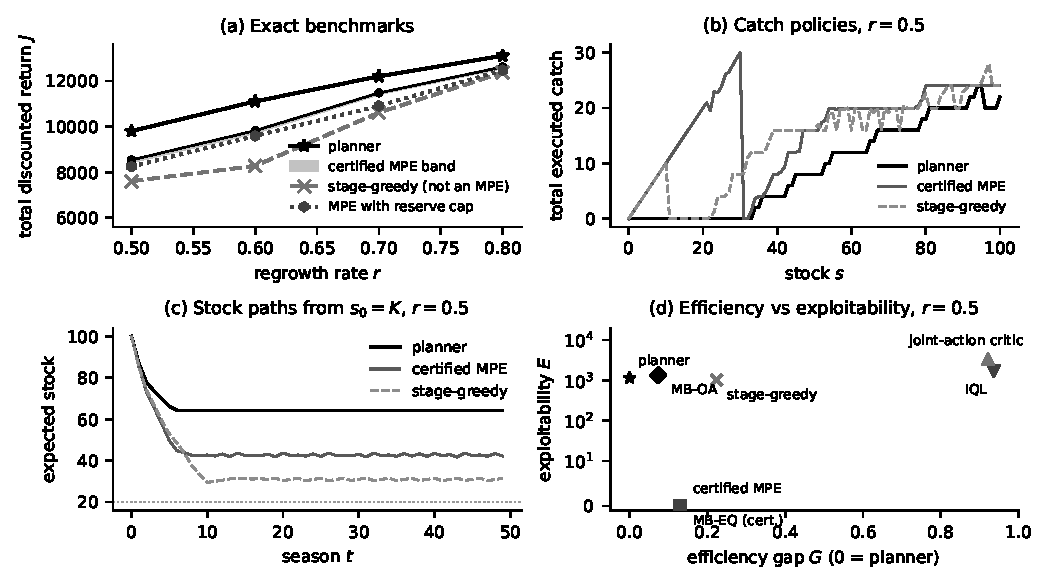
\includegraphics[width=\linewidth]{fig_bench_frontier.pdf}
\caption{(a) Planner, certified MPE band, the stage-greedy profile and the capped (safe) MPE as functions of $r$.
(b) Stationary catch policies and (c) expected stock paths from $s_0=K$ at $r=0.5$ (dotted: collapse threshold $\delta K$).
(d) Every profile and learner at $r=0.5$ by efficiency gap and exploitability (symmetric log scale): the planner is
efficient but exploitable, equilibria are unexploitable but inefficient, MB-OA sits near the planner.}
\label{fig:bench}
\end{figure}

\subsection{Learners in self-play (Q1, Q2)}
Table~\ref{tab:learners} and Figure~\ref{fig:curves} summarise self-play after training. Independent Q-learning ends far
below every equilibrium ($G=0.90$--$0.94$) and the stock collapses in 96--100\% of evaluation runs. Its learning cost
per episode, $\bar L_\tau$ against the planner, is 3.4--4.1 times that of MB-OA. A shared team reward does not help
(Team-IQL $G\approx0.95$), so the failure comes from decentralised exploration, not from selfish incentives. The tabular
joint-action critic is only slightly better ($G=0.78$ at $r=0.8$). MB-EQ reaches exactly the equilibrium it is told to
play: with a certified MPE it gets the MPE value with collapse at most 2\% and $E\le2$; with the stage-greedy profile it
inherits that profile's exploitability and its collapse rate of 38\% at $r=0.6$. MB-OA settles closest to the planner
($G=0.023$--$0.074$, no collapse) in 200 episodes, but in self-play it is exploitable ($E=708$--$1339$): each fleet best
responds to a model of a cooperative-looking opponent, so neither is at an equilibrium.
Patience and noise matter as Q1 anticipated (collapse rates averaged over $r$): with $\gamma=0.90$ MB-EQ collapses the
stock in 90--100\% of runs and with $\sigma=0.2$ in 61\% even at $\gamma=0.99$, whereas MB-OA keeps collapse at or below
0.1\% whenever $\sigma\le0.1$ and at 7\% for $\sigma=0.2$, $\gamma=0.99$.

\begin{table}[h]
\centering
\caption{Self-play after training: $G$ / $C_{50}$ / $E$ (means over 20 seeds; $\gamma=0.99$, $\sigma=0.1$).}
\label{tab:learners}
\small
\begin{tabular}{lcccc}
\toprule
Learner (episodes) & $r=0.5$ & $r=0.6$ & $r=0.7$ & $r=0.8$ \\
\midrule
IQL (5000) & 0.937 / 1.00 / 1{,}714 & 0.936 / 1.00 / 3{,}078 & 0.922 / 0.99 / 4{,}559 & 0.903 / 0.96 / 5{,}774 \\
MB-EQ, certified MPE (500) & 0.130 / 0.02 / 0 & 0.119 / 0.02 / 0 & 0.060 / 0.00 / 1 & 0.041 / 0.00 / 2 \\
MB-EQ, stage-greedy profile (500) & 0.224 / 0.01 / 1{,}030 & 0.255 / 0.38 / 272 & 0.131 / 0.00 / 95 & 0.056 / 0.00 / 11 \\
MB-OA (200) & 0.074 / 0.00 / 1{,}339 & 0.055 / 0.00 / 1{,}246 & 0.045 / 0.00 / 1{,}110 & 0.023 / 0.00 / 708 \\
Joint-action critic (5000) & 0.922 / 0.99 / 3{,}339 & 0.901 / 0.93 / 4{,}944 & 0.870 / 0.84 / 5{,}609 & 0.776 / 0.54 / 5{,}652 \\
Team-IQL (5000) & 0.955 / 1.00 / 1{,}123 & 0.957 / 1.00 / 1{,}799 & 0.958 / 1.00 / 3{,}319 & 0.951 / 1.00 / 4{,}707 \\
\bottomrule
\end{tabular}

\end{table}

\begin{figure}[h]
\centering
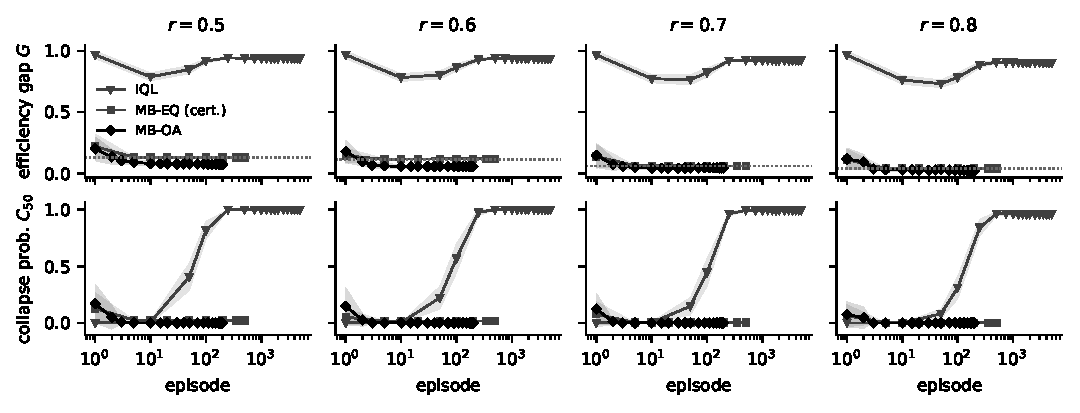
\includegraphics[width=\linewidth]{fig_curves.pdf}
\caption{Learning curves: efficiency gap (top; dotted: best certified MPE) and evaluation collapse probability (bottom),
mean and 95\% interval over 20 seeds.}
\label{fig:curves}
\end{figure}

\subsection{Responding to the other fleet (review feedback 1)}
Table~\ref{tab:cross} pairs MB-OA and MB-EQ against the same opponent, seed and noise. Against an over-harvester MB-OA
lowers its own request and gains $+1436.5\pm331.3$ (pooled), up to $+3702.1$ at $r=0.8$ where MB-EQ collapses the stock.
Against an equilibrium player it loses a little own return (significantly, $-31$ to $-672$, except a gain of $+106$ at
$r=0.6$) while raising joint efficiency ($\Delta G=-0.12$ pooled): it best-responds rather than defends.
Against another MB-OA it earns 1038 less than MB-EQ would (pooled), consistent with its exploitability in
Table~\ref{tab:learners}. Opponent
modelling therefore pays exactly when the opponent departs from the equilibrium.

\begin{table}[h]
\centering
\caption{Paired difference in own return, MB-OA minus MB-EQ, by opponent and $r$ ($^{*}$: Holm-adjusted $p<0.05$, 24 tests).
$^{\dagger}$The IQL opponent trains for 200 episodes when paired with MB-OA but 500 when paired with MB-EQ, so this row is
not a like-for-like comparison.}
\label{tab:cross}
\small
\begin{tabular}{lccccc}
\toprule
Opponent & $r=0.5$ & $r=0.6$ & $r=0.7$ & $r=0.8$ & pooled (95\% CI) \\
\midrule
MB-EQ & -671.5$^{*}$ & +106.5$^{*}$ & -31.0$^{*}$ & -97.9$^{*}$ & -173.5 $\pm$ 69.5 \\
MB-OA & -1{,}540.2$^{*}$ & -1{,}253.6$^{*}$ & -838.6$^{*}$ & -521.3$^{*}$ & -1{,}038.4 $\pm$ 167.5 \\
IQL$^{\dagger}$ & +2.0 & +19.3 & +20.4 & -299.7 & -64.5 $\pm$ 101.9 \\
Planner share & -34.3$^{*}$ & +45.2$^{*}$ & +100.2$^{*}$ & +99.4$^{*}$ & +52.6 $\pm$ 12.3 \\
Stage-greedy profile & -718.8$^{*}$ & +138.3$^{*}$ & -8.1$^{*}$ & -70.7$^{*}$ & -164.8 $\pm$ 74.3 \\
Over-harvester ($a=14$) & +52.5$^{*}$ & +185.2$^{*}$ & +1{,}806.2$^{*}$ & +3{,}702.1$^{*}$ & +1{,}436.5 $\pm$ 331.3 \\
\bottomrule
\end{tabular}

\end{table}

\subsection{Not knowing $r$, and the amount of data (Q3)}\label{sec:unknownr}
The posterior puts all its mass within $0.05$ of the true $r$ in every run. Paired by seed, the first-episode cost of not
knowing $r$ is small ($-44.7\pm33.8$ at $r=0.5$, about 2\% of an episode's return) and not distinguishable from zero at
$r=0.6$ and $0.8$; after that the belief-based and known-$r$ learners are indistinguishable ($G=0.224$ both at $r=0.5$).
The 11.6--18.1\% of runs that collapse during the exploratory warm-up do so equally with and without knowledge of $r$.
The data sweep agrees that the warm-up length is what matters: without warm-up MB-OA training collapse is 0--0.7\%,
against 13.0\% with 5 warm-up seasons and 84.0\% with 50, while the re-planning interval and the prior width change the
final $G$ by at most 0.014.

\textbf{When the true $r$ was never solved.} MB-EQ plays the equilibrium interpolated between the values of $r$ that were
solved in advance, and in all experiments above the true $r$ is one of them. Evaluating exactly the policy MB-EQ converges
to when the true $r$ lies between solved values (E12), at $r=0.55$, $0.65$ and $0.75$ it loses 1.9\%, 1.7\% and 0.7\% of
welfare against the certified MPE at that $r$, and a fleet gains 1.5\%, 0.7\% and 0.3\% of its value by deviating.
Interpolating equilibria is therefore a mild but real approximation; solving at the posterior mean removes it.

\subsection{Safety: what the reserve cap costs (Q3)}
Table~\ref{tab:safety} separates who pays for the reserve cap. The cap never binds for the planner (zero cost). For
selfish fleets it removes the equilibrium's residual collapse risk (up to 3.6\%) but lowers the equilibrium value by
142--563. The capped equilibrium is itself certified (an exact equilibrium at $r=0.5$, an $\varepsilon$-equilibrium with
$\varepsilon\le0.2\%$ of value at $r\ge0.6$). The cap is a safety instrument, not an efficiency one: it does not move
selfish fleets towards the planner. Learners trained under the cap have no collapse in training or evaluation.

\begin{table}[H]
\centering
\caption{Reserve cap ($S_{\text{res}}=25$): planner and best certified MPE without and with the cap, and the MPE collapse rate.}
\label{tab:safety}
\small
\begin{tabular}{cccccccc}
\toprule
 & \multicolumn{2}{c}{Planner} & \multicolumn{2}{c}{Best certified MPE} & Cost of cap & \multicolumn{2}{c}{$C_{50}$ of MPE} \\
$r$ & uncapped & capped & uncapped & capped & (equilibrium) & uncapped & capped \\
\midrule
0.5 & 9{,}802.5 & 9{,}802.5 & 8{,}532.6 & 8{,}246.1 & +286.6 & 0.036 & 0.000 \\
0.6 & 11{,}103.6 & 11{,}103.6 & 9{,}821.2 & 9{,}589.3 & +232.0 & 0.008 & 0.000 \\
0.7 & 12{,}204.1 & 12{,}204.1 & 11{,}474.4 & 10{,}911.5 & +562.9 & 0.004 & 0.000 \\
0.8 & 13{,}106.6 & 13{,}106.6 & 12{,}614.7 & 12{,}472.3 & +142.3 & 0.000 & 0.000 \\
\bottomrule
\end{tabular}

\end{table}

\subsection{Can cooperation be sustained? (Q4)}\label{sec:coop}
\IfFileExists{tables/tab_coop.tex}{%
Table~\ref{tab:coop} and Figure~\ref{fig:coop} give the exact grim-trigger threshold. Cooperation at the planner's
catch \emph{can} be sustained as a subgame-perfect equilibrium: Eq.~\eqref{eq:grim} holds at every stock if and only if
$\gamma\ge\gamma^*(r)$, with $\gamma^*$ between 0.77 ($r=0.5$) and 0.68 ($r=0.8$), far below the $\gamma=0.99$ we study.
The binding stocks are low ones ($s\approx7$--$12$), where the planner lets the stock rebuild and a deviator could take
what is left; a one-season deviation gains little elsewhere because the cost is convex, while punishment loses the value
of cooperation for good. $\gamma^*$ falls as $r$ rises because faster regrowth shortens the rebuilding the cooperative
path asks for. At every $\gamma$ near the threshold the punishment equilibrium passes the certificate ($E\le0.07$).

The learners do not find this cooperation. Under a forced one-season over-harvest, memory-one learners cut their next
catch by 3.3--3.7, but at the same stock their catch after a deviation differs by about one unit or less, and the regime
bit fires by construction (the probe catch is above the trigger threshold). The cut follows the lower stock, not a
learned punishment. Sustaining cooperation therefore requires the strategy to be designed or computed, not discovered by
tabular Q-learning in 5000 episodes.
\begin{figure}[h]
\centering
\begin{minipage}[c]{0.40\linewidth}
\centering
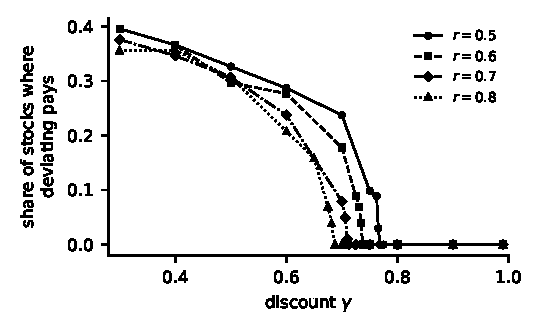
\includegraphics[width=\linewidth]{fig_coop.pdf}
\captionof{figure}{Share of stocks at which a one-season deviation from cooperation pays, against $\gamma$. Zero means
the grim trigger is a subgame-perfect equilibrium.}
\label{fig:coop}
\end{minipage}\hfill
\begin{minipage}[c]{0.57\linewidth}
\centering
\captionof{table}{Exact grim-trigger threshold (cooperation = symmetric planner, punishment = certified MPE) and the
memory-one probe (same-stock catch after a deviation minus without; negative = restraint).}
\label{tab:coop}
\scriptsize
\begin{tabular}{cccc}
\toprule
$r$ & $\gamma^*$ (SPE iff $\gamma\ge\gamma^*$) & $J^{\text{coop}}-J^{*}$ ($\gamma=0.99$) & memory-one gap \\
\midrule
0.5 & 0.767 $\pm$ 0.002 & +1{,}266.6 & -1.29 $\pm$ 1.12 \\
0.6 & 0.736 $\pm$ 0.002 & +1{,}279.3 & -1.00 $\pm$ 0.94 \\
0.7 & 0.711 $\pm$ 0.002 & +725.2 & -0.12 $\pm$ 0.78 \\
0.8 & 0.684 $\pm$ 0.003 & +518.8 & -0.24 $\pm$ 1.20 \\
\bottomrule
\end{tabular}

\end{minipage}
\end{figure}}{}

\subsection{Answers and limitations}
\textbf{Q1:} independent learners settle far below any equilibrium; model-based learners reach the equilibrium they
play; opponent-aware learners settle near the planner but are exploitable. \textbf{Q2:} a model plus exact planning
matters more than a centralised critic: MB-OA has a 3.4--4.1$\times$ lower learning cost than IQL, and the joint-action
critic barely improves on IQL. \textbf{Q3:} not knowing $r$ costs little once the belief is used. The warm-up exploration,
not the uncertainty, causes collapse during learning, and a reserve cap removes collapse at a welfare cost borne only by
selfish play. \textbf{Q4:} cooperation is sustainable as a subgame-perfect equilibrium for $\gamma\ge\gamma^*\approx0.68$--$0.77$,
but memory-one learners do not learn it.
\textbf{Limitations.} Two fleets only (three fleets and the neural actor-critic, planned as optional extensions, were not run); a stylised growth law;
grid discretisation (a finer catch grid moves the certified equilibrium value by under 2\%); symmetric mixed equilibria
are enumerated only with support size 2; independent learners have no convergence guarantee (their non-convergence is
reported as a result); the learning experiments use true $r$ values that were solved in advance (Section~\ref{sec:unknownr}
measures the cost otherwise); the IQL opponent's training budget differs between the two compared learners in
Table~\ref{tab:cross}.
